188. \begin{figure}[ht!]
\center{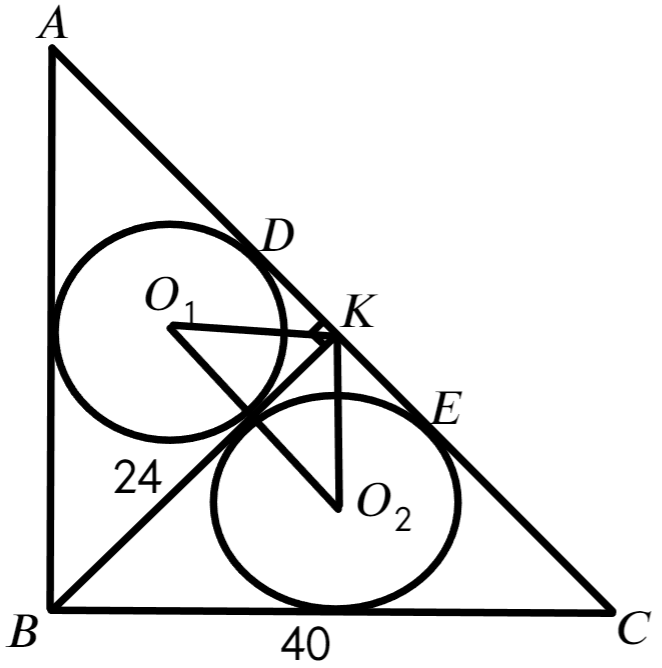
\includegraphics[scale=0.35]{g9-188.png}}
\end{figure}\\
По теореме Пифагора $KC=\sqrt{40^2-24^2}=32.$ Пусть $AB=x,\ AK=y,$ тогда имеет место система уравнений $\begin{cases}x^2+1600=(y+32)^2,\\
y^2+576=x^2.\end{cases}\Leftrightarrow\begin{cases}x^2+1600=y^2+64y+1024,\\
x^2-y^2=576.\end{cases}\Leftrightarrow\begin{cases}576=64y-576,\\
x^2-y^2=576.\end{cases}\Leftrightarrow\begin{cases}y=18,\\
x^2-324=576.\end{cases}\Leftrightarrow\begin{cases}y=18,\\
x=30.\end{cases}$ Найдём радиус окружности, вписанной в треугольник $ABK:\ S_{\Delta ABK}=\cfrac{1}{2}\cdot24\cdot18=r\cdot\cfrac{24+30+18}{2},$ откуда $r=6.$ Пусть эта окружность касается стороны $AK$ в точке $D,$ тогда $DK=\cfrac{24+18-30}{2}=6$ и $KO_1^2=6^2+6^2=72.$ Аналогично для треугольника $BKC:\ S_{\Delta BKC}=\cfrac{1}{2}\cdot24\cdot32=R\cdot\cfrac{24+32+40}{2},$ откуда $R=8,\ EK=\cfrac{24+32-40}{2}=8,\ KO_2^2=8^2+8^2=128.$ Так как $KO_1$ и $KO_2$ являются биссектрисами, имеем равенство $\angle O_1KO_2=\angle O_1KB+\angle BKO_2=45^\circ+45^\circ=90^\circ$ и по теореме Пифагора $O_1O_2^2=KO_1^2+KO_2^2=72+128=200,\ O_1O_2=10\sqrt{2}.$\\
